% This syllabus template was created by:
% Brian R. Hall
% Assistant Professor, Champlain College
% www.brianrhall.net
% and then adapted by:
% Kyle N. Winfree
% Associate Professor, Northern Arizona University
% winfreelab.nau.edu

% Document settings
\documentclass[11pt]{article}
\usepackage[margin=1in]{geometry}
\usepackage{graphicx}
\usepackage{wrapfig}
\usepackage{multirow}
\usepackage{setspace}
\usepackage{hyperref}
\usepackage{xurl}
\usepackage{booktabs}
\pagestyle{plain}
\setlength\parindent{0pt}

\begin{document}

\Huge INF632 Syllabus
\normalsize ~

\noindent\rule{\textwidth}{1pt}\vspace{.5em}

\LARGE Topics in Wearable Computing
\normalsize ~

% Course information
\begin{description}
	\item [College:] Steve Sangi College of Engineering (SCE)
	\item [Department:] School of Informatics, Computing, and Cyber Systems
	\item [Course-Section Number:] INF632-000 (this semester as EE499-100 and EE599-100)
	\item [Time:] Tuesdays and Thursdays, 11:10am to 12:25pm
	\item [Location:] Class will meet SICCS (90) Room 223, and occasionally SICCS 122
	\item [Lecture / Hands On Lab:] January 12 to May 1, 2026
	\item [Final Presentations:] In finals week, Thursday May 7 10:00am to 12:00pm
	\item [Credit Hours:] 3 (Co-convened this semester)
	\item [Prerequisite(s):] Graduate Status (None for EE499 and EE599)
	\item [Modality:] Face-to-face
	\item [Course Website:] \href{https://canvas.nau.edu}{canvas.nau.edu}, \href{https://github.com/kylewinfree/inf632-spring2026}{github.com/kylewinfree/inf632-spring2026}
\end{description}
%\vspace{2em}

% Professor information
\begin{tabular}{ l l }
	\multirow{6}{*}{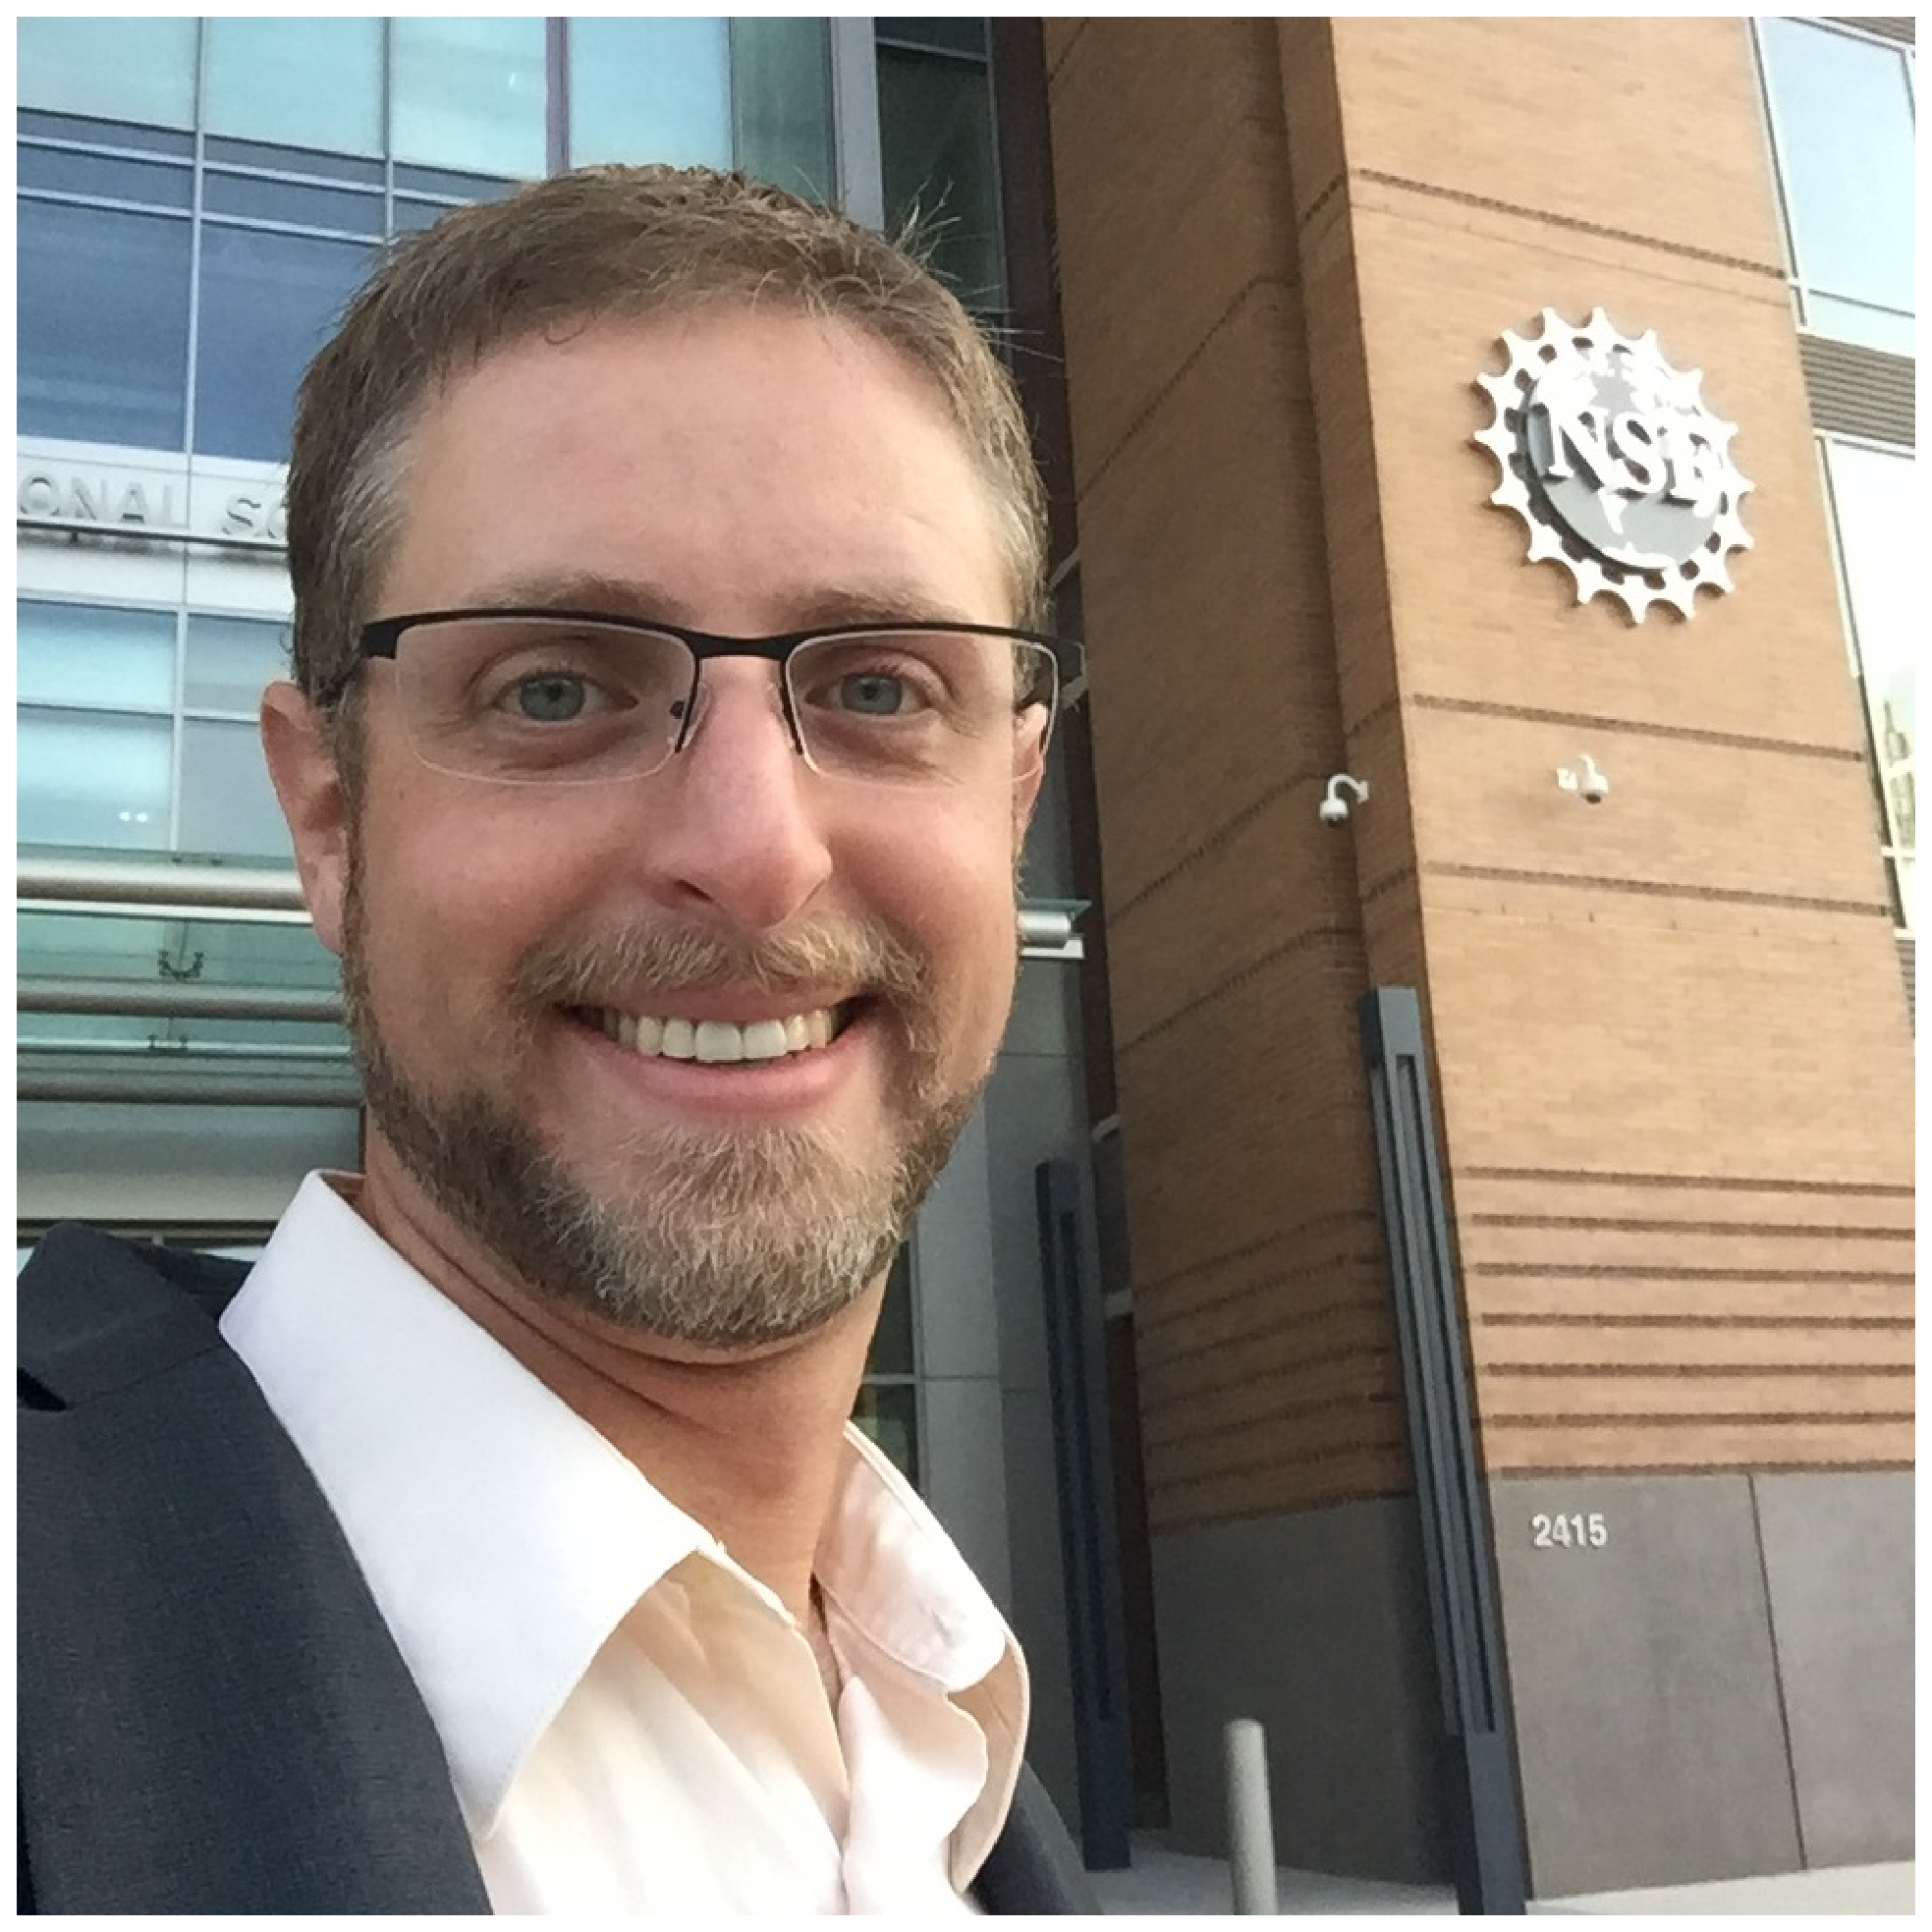
\includegraphics[height=1.5in, width=1in]{kyle.eps}} & Kyle N. Winfree \\
	& \href{mailto:kyle.winfree@nau.edu}{kyle.winfree@nau.edu} \\
	& \href{https://winfreelab.nau.edu}{winfreelab.nau.edu} \\
	& SICCS (90) Room 204 \\
	& Office Hours: Thursdays 12:45-2:00 and Mondays 1:00-2:00 \\
	& Cell Phone: 928.853.0114, please use sparingly - I will not respond during class!
\end{tabular}
\vspace{2em}

\begin{center} This syllabus is subject to change at the discretion of the instructor. \\
\end{center}

% Course details
\section*{Academic Catalog Description:} Study of methods, techniques, and research areas in wearable computing, with varying emphases between offerings. Letter grade only. May be repeated for up to 6 unis of credit with different topic.

\section*{Course Description:} This project-based course is intended to provide a graduate-level study of wearable technologies, including the use of commercially available devices, such as the Fitbit. The course centers on the client-host interface and data exchanges involved in the design and application of wearable technologies, with a particular focus on applications in healthcare and wellness. Topics include applications of wearable technologies in health research, comparative studies, projects involving the creation of custom health monitoring devices, data analysis, real-time analysis techniques, and machine learning. Students will engage in iterative design projects that explore and apply a variety of wearable technology techniques and scholarly literature reviews that explore open research areas in the field. By the end of the course, students are able to engage in research in wearable computing and the design and creation of wearable devices in other research areas of interest.

\section*{Course Student Learning Outcomes:}
\subsection*{Undergraduate:}
Students who complete the undergraduate section of this course in good standing should be able to demonstrate the following advanced competencies:
\begin{enumerate}
	\item Select, assess, and apply techniques appropriate to the application of wearable technologies for healthcare and wellness applications;
	\item Synthesize, apply, and evaluate offline data analysis and machine learning techniques on large-scale data sets collected by wearable technologies;
	\item Identify, interpret, and critically explain the significance of open research areas in wearable technologies and their applications in health-driven research;
	\item Evaluate the applicability of wearable technologies in the commodity market.
\end{enumerate}

\subsection*{Graduate:}
Students who complete the graduate section of this course in good standing should be able to demonstrate the following advanced competencies:
\begin{enumerate}
	\item Select, assess, and apply techniques appropriate to the design and implementation of wearable technologies for healthcare and wellness applications, including specialized communication protocols and data structures and storage techniques;
	\item Synthesize, apply, and evaluate online and offline data analysis and machine learning techniques on large-scale data sets collected by wearable technologies;
	\item Identify, interpret, and critically explain the significance of open research areas in wearable technologies and their applications in health-driven research;
	\item Evaluate the applicability of wearable technologies in the commodity and research.
\end{enumerate}


\section*{Assessment of Student Learning Outcomes:} %Assignments/Assessments of Course Student Learning Outcomes. Articulates key assignments/assessments that will be used to provide clear indications of student achievement of course Student Learning Outcomes, and provides a summary of the purpose and description of the assignments/assessments.
Methods of assessment include: reading and homework assignments; participation in the in-class reading discussions; and a research project (purpose statement; literature review; implementation and comparison of several machine learning algorithms; final project report) in stages throughout the semester. Evaluations of the team project will be done at an individual level. Students will be required to complete their own literature review, hypothesis formation, and analysis/discussion of results. While the research methods plan and device design/implementation are dependent on other team members and will have a strong group influence, students will need to justify their own contributions and independently propose alternative designs and methods.

\section*{Grading System:} %Grading System. Includes such elements as how points or percentages will be allocated to each assignment/ assessment, points or percentages necessary to achieve each letter grade, etc.
This is a project heavy course. You will work through conception, development, implementation, and reflective analysis of a project in wearable computing. This project may include hardware development, will very likely include numerical analysis, and will absolutely include a formal written report and presentation. You may elect to work individually, or in a team of two. However, the scope of the project must be appropriate for either of these options - meaning, a team of two will have higher expectations than that of a person working individually.  The relative impact of each assessment in your final grade can be found in Table~\ref{tab:percentage}. Final course letter grades will be determined as shown in the Table~\ref{tab:letter}.  There is no ``curve;'' your grade is completely up to you and is not affected by the grades of your classmates. Extra credit opportunities may present themselves throughout the semester and be announced during class meetings. If you feel a mistake has been made in grading your assignment, please address your concerns during office hours.

Graduate students will be graded with a different rubric than undergraduate students and in general will be expected to do more.  As your instructor, I expect to have access to all materials related to your assignments.  This includes data, design files, analyses, and write ups.
\subsection*{Undergraduate:}
Undergraduate students may use either GitHub or Google Drive to share all work with the instructor.  Both support Colab, which undergraduate students are encouraged to use for analysis and report generation.  These students may complete assignment write ups in Google Docs (recommended) or \LaTeX.  Write ups must then be exported to pdf\footnote{\url{https://dev.to/revisepdf/the-history-of-pdf-from-adobes-creation-to-universal-standard-33d}}.
\subsection*{Graduate:}
Graduate students must use GitHub to share all work with the instructor.  All analysis code (Octave, Python / Jupyter Notebooks, or R) must be available in this repository.  All written assignments must be submitted typeset in IEEE BHI \LaTeX format\footnote{\url{https://template-selector.ieee.org/secure/templateSelector/publicationType}} (not MS Word, Pages, Google Docs, or chicken scratch).

\begin{table}
    \begin{center}
    \caption{Assessments and related fractional percentage of final grade.\label{tab:percentage}}
        \begin{tabular}{lcc}
            \textbf{Assessment}									& \textbf{Undergraduate} & \textbf{Graduate} \\
            \toprule
            Attendance and in-class participation 				& 10\%			& 10\%\\
            \midrule[0.01em]
            Homework Assignments (3) 							& 45\% 			& 30\% \\
            \midrule[0.01em]
            Research Project: Literature Review 				& 5\% 			& 10\% \\
            Research Project: Questions and Hypotheses 			& 10\% 			& 10\% \\
            Research Project: Device Design and Implementation 	& 5\% 			& 10\% \\
            Research Project: Methods Plan 						& 5\% 			& 5\% \\
            Research Project: Analysis 							& 5\% 			& 10\% \\
            Research Project: Discussion of Findings 			& 10\% 			& 10\% \\
            Research Project: In-Class Presentation 			& 5\% 			& 5\% \\
            \bottomrule
            Total												& 100\%			& 100\%
        \end{tabular}
    \end{center}
\end{table}


\begin{table}
\begin{center}
\caption{Percentage grade and corresponding letter grade.\label{tab:letter}}
\begin{tabular}{cc}
\textbf{Percentage Grade} ($G$) 	& \textbf{Letter Grade} \\
\toprule
$G \geq 90\%$			& A \\
$90\% > G \geq 80\%$	& B \\
$80\% > G \geq 70\%$	& C \\
$70\% > G \geq 60\%$	& D \\
$60\% > G $				& F \\
\end{tabular}
\end{center}
\end{table}

\section*{Readings and Materials:} No text book will be required. You will need to purchase the materials to create a wearable device. This material list will be provided; expect costs to be approximately that of a textbook.  Students in the undergraduate section have the option of completing the research project with off-the-shelf devices and may not need to purchase materials.  Additional readings will be provided from various sources; this list below includes materials that will not be provided to you in class and are recommended as helpful readings. % https://www.youtube.com/watch?v=PygUK16aQgk
\begin{enumerate}
\item \emph{Open Software, Second Edition}, by Tony Olsson, David Gaetano, Samson Wiklund, \& Jonas Odhner (ISBN: 978-91-97-95540-9)
\item \emph{Practical Arduino}, by Jonathan Oxer and Hugh Blemings (ISBN: 978-1430224778)
\item \emph{GNU Octave - A high-level interactive language for numerical computations}, by John W. Eaton~\footnote{\url{https://www.octave.org/}}
\item \emph{Python Data Science Handbook}, by Jake VanderPlas (ISBN:978-1-491-91205-8) 
\item \emph{R: A Language and Environment for Statistical Computing - The R Manuals}, by the R Core Team~\footnote{\url{https://www.r-project.org/}}, \footnote{\url{https://cran.r-project.org/manuals.html}}
\item \emph{\LaTeX}~\footnote{\url{https://en.wikibooks.org/wiki/LaTeX}}, \footnote{\url{https://upload.wikimedia.org/wikipedia/commons/2/2d/LaTeX.pdf}}
\end{enumerate}

% https://journals.ieeeauthorcenter.ieee.org/create-your-ieee-journal-article/authoring-tools-and-templates/tools-for-ieee-authors/ieee-article-templates/




% Course Policies. These are just examples, modify to your liking.
%\newpage % because I don't like how the itemize is breaking.  Maybe I should have used subsection...
\section*{Course Policies}
\begin{itemize}
	\item \textbf {Your Work should be Your Work}
		\begin{itemize}
			\item Cheating and plagiarism are strictly prohibited. All academic integrity violations are treated seriously. All work you submit for grading must be your own. You are encouraged to discuss the intellectual aspects of assignments with other class participants. However, each student is responsible for formulating responses and solutions on their own and in their own words.  Academic integrity violations will result in penalties including, but not limited to, a zero on the assignment, a failing grade in the class, or expulsion from NAU or your degree program.
		\end{itemize}
	\item \textbf{Generative Artificial Intelligence}
		\begin{itemize}
			\item I'd like you to know that I am not strictly opposed to the use of generative AI.  However, I want to see you use it appropriately.
			\item Written reports or explanations of your work that are indicative of generative AI may be considered cheating.  This doesn't mean that you can't use something like Grammarly to help you improve your writing, but this does mean that you shouldn't ask a generative AI to summarize your code for you.
			\item We all run into challenges when coding at times.  You may certainly ask your friend, your favorite search engine, or a generative AI to help you through a bug or to figure out what functions/methods you should be using.  You should not however be copy-pasting code from generative AI into your code.  Instead, consider this: copy-paste the prompt or search term and the key response from either into a comment block.  Then, use that to help you write your own code!
			\item The bigger problem with using generative AI, in my opinion, isn't that you could be learning to copy-paste, but is instead that YOU AREN'T LEARNING\footnote{\url{https://www.youtube.com/watch?v=G-cdVurdoeA}}.  You're hear to learn.  Sure, maybe also to earn a degree and then get a job, but you won't likely be able to maintain that job if you haven't actually learned what your degree says you did.  Don't cheat yourself out of your education.
		\end{itemize}
	\item \textbf{Be Present}
		\begin{itemize}
			\item Electronic device usage must support learning in the class.  This includes notebook computers, tablets, and phones.
			\item I devote 100\% of my attention to providing a high-quality lecture; please respect this by devoting 100\% of your attention to listening and participating.
		\end{itemize}
	\item \textbf {Grades\footnote{\url{https://www9.nau.edu/policies/Client/Details/1996}}}
		\begin{itemize}
			\item For those in the undergraduate section, a \textbf{C} grade reflects \textbf{average} performance, a \textbf{B} grade reflects \textbf{above average}, and an \textbf{A} grade reflects work that is \textbf{excellent}.
			\item For those in the graduate section, a \textbf{C} grade is the \textbf{lowest grade acceptable for graduate credit} and may trigger academic probation, a \textbf{B} grade reflects performance that is \textbf{satisfactory}, and an \textbf{A} grade reflects work that is \textbf{superior}.
			\item Grades will be maintained in the Canvas LMS course shell. Students are responsible for tracking their progress by referring to the online grade book and cross referencing to the course materials.
			\item There is no course grading curve, but the grading rubric may be adjusted in cases where all students are observed to have struggled.
		\end{itemize}
	\item \textbf{Attendance and Absences}
		\begin{itemize}
			\item Attendance is expected. Regular absences and non-participation may result in the reduction of your final grade by up to one letter grade. If you expect to be absent, please notify me, your instructor.  The same goes for absences resultant of sickness or other emergencies.
			\item Students are responsible for all missed work, regardless of the reason for absence. It is also the absentee's responsibility to get all missing notes or materials. 
		\end{itemize}
	\item \textbf{Communication}
		\begin{itemize}
			\item Emails and Canvas messages to the instructor and teaching assistants must be respectful and professional.  Specifically, such messages should adhere to the following:
			\begin{itemize}
				\item Contain a salutation, (for example, ``Dear Dr. Winfree,'' or ``Kyle,'')
				\item Contain a closing, (for example, ``Best, Jane Doe'')
				\item The body should contain complete sentences and correct grammar including correct usage of lowercase and uppercase letters. Composing emails on a mobile device is not an excuse for poor writing. Poorly composed emails may be returned without a response to the questions asked.
				\item The body of your message should also be respectful and explain the full context of the query.  If you are asking for input on any of your assignment materials, be sure to include a link to your repository.
				\item The subject should be prefixed with ``INF632'' so that the message can be easily identified   or placed in an auto-folder. The subject should also use lower case and upper case correctly.
			\end{itemize}
			\item Please allow up to three business days for a response to email.  To accelerate this timeline, please send your message via Canvas - this will pop up on my phone right away.  My cell number is provided above.  I ask that this be used sparingly and for reasonable emergencies.
			\item If you have a question that would require a long response or you have a lot of questions, please come to office hours or schedule an appointment with the instructor or teaching assistant.
			\item Visiting during office hours is encouraged! I am happy to talk about the class, careers, research, and topics related (even loosely) to this course.
		\end{itemize}
\end{itemize}
\section*{University Policies}
The University Policy Library contains the Syllabus Policy Statements\footnote{\url{https://nau.edu/university-policy-library/syllabus-requirements/}} in addition to many other relevant and important policies.

\newpage
\section*{Tentative Schedule:} % Class Outline or Tentative Schedule. Includes expectations regarding the class schedule; when assignments, readings, materials, etc. need to be completed; and expectations about completing work, lab, or field trip requirements across the term within which the section is taught.
Shown in Table~\ref{tab:schedule} outlines a tentative schedule.  This may be adjusted for a variety of reasons, such as supporting your learning and instructor conflicts.
\begin{table}[ht!]
\begin{center}
\caption{Tentative Course Schedule.\label{tab:schedule}}
\begin{tabular}{c p{4in}}
\textbf{Week of} & \textbf{Content} \\
\toprule

% this tex file includes the defs for due dates, making it possible to update this file each semester and have all the dates automatically reflect in all docs.

% pgfmath might be a better approach.
% or a python script that takes a few inputs and then generates this file.

% week 1
\def \wkOneMo{January 12} % course intro, reading
\def \wkOneTu{January 13}
\def \wkOneTh{January 15} % HW1 assigned

% week 2
\def \wkTwoMo{January 19} % this is generally MLK day
%                           dims of func, hapitcs
\def \wkTwoTu{January 20}
\def \wkTwoTh{January 22}

% week 3
\def \wkThreeMo{January 26} % health trends, analysis, compare testing
\def \wkThreeTu{January 27}
\def \wkThreeTh{January 29} % HW1 due, HW2 assigned

% week 4
\def \wkFourMo{February 2} % intro of RP, res methods for studies
\def \wkFourTu{February 3}
\def \wkFourTh{February 5}

% week 5
\def \wkFiveMo{February 9} % Lit rev, hypothesis, no class Thurs (2026)
\def \wkFiveTu{February 10} % RP-lit review assigned
\def \wkFiveTh{February 12}

% week 6
\def \wkSixMo{February 16} % Statistical learning, regression, fitting, NNs
\def \wkSixTu{February 17}
\def \wkSixTh{February 19} % HW2 due, HW3 assigned

% week 7
\def \wkSevenMo{February 23} % Stat Learn SVM, trees, k-means, knn
\def \wkSevenTu{February 24} % RP-lit review due, RP-Q&H assigned
\def \wkSevenTh{February 26}

% week 8
\def \wkEightMo{March 2} % device design, sensing
\def \wkEightTu{March 3} % RP-Q&H due, RP-design assigned
\def \wkEightTh{March 5}

% spring break
\def \springBreakMo{March 9} % NADA
\def \springBreakFr{March 13} % RIEN
%\def \springBreakTh{March 12}

% week 9
\def \wkNineMo{March 16} % soldering lab, arduino pt 1
\def \wkNineTu{March 17}
\def \wkNineTh{March 19} % HW3 due

% week 10
\def \wkTenMo{March 23} % arduino pt 2, raspberry pi
\def \wkTenTu{March 24} % RP-design due, RP-methods assigned
\def \wkTenTh{March 26}

% week 11
\def \wkElevenMo{March 30} % project time
\def \wkElevenTu{March 31} % RP-methods due, RP-analysis assigned
\def \wkElevenTh{April 2}

% week 12
\def \wkTwelveMo{April 6} % project time
\def \wkTwelveTu{April 7}
\def \wkTwelveTh{April 9}

% week 13
\def \wkThirteenMo{April 13} % interp results, communicating findings
\def \wkThirteenTu{April 14} % RP-analysis due, RP-discuss assigned
\def \wkThirteenTh{April 16}

% week 14
\def \wkFourteenMo{April 20} % writing lab
\def \wkFourteenTu{April 21} % RP-discuss due, RP-pres assigned
\def \wkFourteenTh{April 23}

% week 15
\def \wkFifteenMo{April 27} % project time
\def \wkFifteenTu{April 28} %RP-pres due
\def \wkFifteenTh{April 30}

% week 16 - Finals Week
\def \finalsWeekMo{May 4}
\def \finalsDay{May 7}
\def \finalsTime{10:00am to 12:00pm}
% \def \wk16Th{January 15}


% January %%%%%%%%%%%%%%%%%%%%%%%%%%%%%%%%%%%%%%%%%%%%%%% Week 1
	January 12 & \begin{minipage}{4in}
	Course expectations, setup (GitHub or Google Drive), and peer introductions (come prepared to introduce yourself with something you learned this past semester or summer).\\
	Start your assigned reading --- this should become habit!
	\end{minipage} \\
	\midrule[0.01em]
%%%%%%%%%%%%%%%%%%%%%%% Week 2
	January 19 & \begin{minipage}{4in}
	Dimensions of functionality\\
	Haptic interfaces\\
	\em{NAU is closed on Monday in observance of MLK Day}
	\end{minipage} \\
	\midrule[0.01em]
%%%%%%%%%%%%%%%%%%%%%%% Week 3
	January 26 & \begin{minipage}{4in}
	Health research and trends in wearable health monitoring\\
	Analysis, comparative testing
	\end{minipage} \\
	\midrule[0.01em]
% February %%%%%%%%%%%%%%%%%%%%%%%%%%%%%%%%%%%%%%%%%%%%%%% Week 4
	February 2 & \begin{minipage}{4in}
	Introduction of the {\bf Research Project}\\
	Research methods for studies\\
	\end{minipage} \\
	\midrule[0.01em]
%%%%%%%%%%%%%%%%%%%%%%% Week 5
	February 9 & \begin{minipage}{4in}
	Literature review, finding the gap in knowledge, forming a hypothesis\\
	No class on Thursday!
	\end{minipage} \\
	\midrule[0.01em]
%%%%%%%%%%%%%%%%%%%%%%% Week 6
	February 16 & \begin{minipage}{4in}
	Statistical learning methods (applied) --- regression, logistic regression, over fitting, neural nets
	\end{minipage} \\
	\midrule[0.01em]
%%%%%%%%%%%%%%%%%%%%%%% Week 7
	February 23 & \begin{minipage}{4in}
	Statistical learning methods (applied) --- support vector machines, decision trees, k-means, k-nearest neighbors
	\end{minipage} \\
	\midrule[0.01em]
%%%%%%%%%%%%%%%%%%%%%%% Week 8
	March 2 & \begin{minipage}{4in}
	Device design\\
	Sensing\\
	\end{minipage} \\
	\midrule[0.01em]
% March %%%%%%%%%%%%%%%%%%%%%%%%%%%%%%%%%%%%%%%%%%%%%%%
	March 9 & \begin{minipage}{4in}
	Spring Break! No class.
	\end{minipage} \\
	\midrule[0.01em]
%%%%%%%%%%%%%%%%%%%%%%% Week 9
	March 16 & \begin{minipage}{4in}
	Soldering lab\\
	Arduino Part 1\\
	Device design review (everyone shares)
	\end{minipage} \\
	\midrule[0.01em]
%%%%%%%%%%%%%%%%%%%%%%% Week 10
	March 23 & \begin{minipage}{4in}
	Arduino Part 2\\
	Raspberry Pi
	\end{minipage} \\
	\midrule[0.01em]
%%%%%%%%%%%%%%%%%%%%%%% Week 11
	March 30 & \begin{minipage}{4in}
	Project time
	\end{minipage} \\
	\midrule[0.01em]
% April %%%%%%%%%%%%%%%%%%%%%%%%%%%%%%%%%%%%%%%%%%%%%%% Week 12
	April 6 & \begin{minipage}{4in}
	Project time
	\end{minipage} \\
	\midrule[0.01em]
%%%%%%%%%%%%%%%%%%%%%%% Week 13
	April 13 & \begin{minipage}{4in}
	Interpreting your results\\
	Communicating your analyses and findings
	\end{minipage} \\
	\midrule[0.01em]
%%%%%%%%%%%%%%%%%%%%%%% Week 14
	April 20 & \begin{minipage}{4in}
	Writing lab --- come prepared to work on writing up the {\bf Discussion and Findings} with your group
	\end{minipage} \\
	\midrule[0.01em]
%%%%%%%%%%%%%%%%%%%%%%% Week 15
	April 27 & \begin{minipage}{4in}
	Project time
	\end{minipage} \\
	\midrule[0.01em]
% May %%%%%%%%%%%%%%%%%%%%%%%%%%%%%%%%%%%%%%%%%%%%%%% Finals Week
	May 4 & \begin{minipage}{4in}
	Finals week, no class on Tuesday\\
	Project presentations on Thursday from 10:00am to 12:00pm
	\end{minipage} \\
	\midrule[0.01em]
\end{tabular}
\end{center}
\end{table}


\end{document}
